\documentclass[12pt]{article}

\usepackage{scrextend}
\usepackage{sbc-template}
\usepackage{mathtools}
\usepackage{subfigure}
\usepackage{wrapfig}
\usepackage{graphicx,url}
\usepackage{booktabs}
\usepackage[brazil]{babel}   
\usepackage[utf8]{inputenc}
\usepackage{hhline}
\usepackage{enumitem, array}
\usepackage{boldline}
\usepackage{hyperref}
\usepackage{url}
\usepackage{relsize}
\usepackage{setspace}
\usepackage[T1]{fontenc} % hifenizar as palavras

\newcommand{\mn}[1]{\textcolor{red}{\bf [Michele]: #1}}

% algoritmo - pacote 9/out/2017
\usepackage[portuguese,ruled,noline,linesnumbered]{algorithm2e}

\let\oldnl\nl% Store \nl in \oldnl
\newcommand{\nonl}{\renewcommand{\nl}{\let\nl\oldnl}}% Remove line number for one line

%% Useful packages
\usepackage{mathtools}
\usepackage{graphicx}
\setlength{\marginparwidth}{2cm}
\usepackage[colorinlistoftodos]{todonotes}
\usepackage{multirow}
\usepackage{bigstrut}

\definecolor{ao(english)}{rgb}{0.0, 0.5, 0.0}

\renewcommand\thesubfigure{(\alph{subfigure})}

\newcommand{\notered}[1]{\textcolor{red}{{#1}}}
\newcommand{\noteblue}[1]{\textcolor{blue}{{\bf #1}}}
\newcommand{\as}[1]{\textcolor{blue}{{\bf #1}}}
\newcommand{\al}[1]{\textcolor{brown}{{\bf #1}}}
\newcommand{\noteMat}[1]{\textcolor{cyan}{{\bf #1}}}
\newcommand{\noteGreen}[1]{\textcolor{green}{{\bf #1}}}
\newcommand{\sep}{\hspace{8 mm}}
\newcommand{\pl}[1]{{\color{red}{[#1]}}}
\newcommand{\mnr}[1]{{\color{blue}{[Necessário corrigir/revisar:  #1]}}}
\newcommand{\co}[1]{{\color{magenta}{[Comentário:  #1]}}}
\newcommand{\mnc}[1]{{\color{brown}{[Comentário:  #1]}}}
\newcommand{\mic}[1]{\textcolor{magenta}{{\bf #1}}}

\definecolor{auburn}{rgb}{0.43, 0.21, 0.1}
\newcommand{\agn}[1]{\textcolor{auburn}{#1}}

\newcommand{\rev}[1]{\textcolor{black}{{#1}}}
%\newcommand{\rev}[1]{\textcolor{red}{{#1}}}

\usepackage{indentfirst}
\usepackage{verbatim}
\usepackage{amsmath}
\sloppy

\usepackage{array}
\usepackage{threeparttable}
\usepackage{listings}

\title{Disseminação Segura de Dados Pessoais Vitais Para Apoio às Tomadas de Decisão em Situações Emergenciais}

\author{Agnaldo de Souza Batista\inst{1}\thanks{{Dissertação de mestrado disponível em https://www.acervodigital.ufpr.br/handle/1884/62473}}\,\,, Aldri Santos\inst{1} (Orientador)} 
\address{Núcleo de Redes Sem-Fio e Redes Avançadas (NR2) -- PPGInf -- UFPR 
\email{\{asbatista,aldri\}@inf.ufpr.br}
}


\usepackage{xcolor}
\usepackage{xwatermark} 
\usepackage[export]{adjustbox}
%\newwatermark*[allpages,angle=60,scale=2,color=red!30,xpos=-10pt,ypos=10pt]{Rascunho}
%\newwatermark[allpages,scale=8,angle=60,xpos=-1.5cm,ypos=1cm]{\LaTeX}
%\newwatermark[allpages,scale=2,angle=60,xpos=-1.5cm,ypos=1cm]{Draft SBRC 2019}

% adicionado por Aldri para inclusão de comentários de pontos a ser melhorados ao longo do documento
%\newcommand{\notered}[1]{\textcolor{red}{[{\bf #1}]}}
%\newcommand{\noteblue}[1]{\textcolor{blue}{{\bf #1}}}
% adicionado por aldri
%\usepackage[inline]{trackchanges}
%\addeditor{FM}
%\addeditor{AS}
%\addeditor{JS}
%%\note[FM]{}

\usepackage{float}

\begin{document} 
\pagestyle{myheadings} % numerar páginas
\maketitle

\begin{abstract}
Urban wireless networks established dynamically have become possible the quick dissemination of a number of data, making them a promising means to support services that require a prompt response. Network health services (\textit{e-health})
%that manage critical health events external to hospital environments and demand dissemination of sensitive personal data
can benefit from interactions in these networks, 
%collaborating in 
anticipating
%specific 
actions to be taken by trained people close to the events until the attendance by the competent health agencies. This dissertation presents the \mbox{STEALTH} system, which employs social trust~and communities of interest to control the dissemination of people's sensitive data in emergencies in dynamic environments. An evaluation of \mbox{STEALTH} under a realistic environment has shown its effectiveness in anticipating the identification of people close to assist in critical health events and the reliability for the dissemination of sensitive data of people in an emergency.

\end{abstract}


\begin{resumo} 

As redes urbanas estabelecidas dinamicamente têm possibilitado a disseminação de dados de maneira rápida, tornando-se um meio promissor ao suporte de serviços que exigem pronta resposta. Os serviços de saúde em redes (\textit{e-health}) 
%que gerenciam eventos críticos de saúde externos aos ambientes hospitalares e demandam a disseminação de dados pessoais sensíveis 
podem se beneficiar das interações nessas redes, 
%colaborando na antecipação de 
%\agn{antecipando} certas ações por pessoas capacitadas 
e possibilitar ações antecipadas por pessoas capacitadas próximas aos eventos até o atendimento pelos órgãos de saúde competentes. Esta dissertação apresenta o sistema \mbox{STEALTH}, 
%um sistema 
que emprega confiança social e comunidades de interesse no controle da disseminação dos dados sensíveis das pessoas em situações emergenciais em ambientes dinâmicos. Uma avaliação do \mbox{STEALTH} num ambiente realístico mostrou a sua eficácia ao antecipar a identificação de pessoas próximas para auxiliar em eventos críticos de saúde, e a sua confiabilidade na disseminação controlada dos dados sensíveis das pessoas em situação emergencial.

\end{resumo}

\section{Introdução}

As redes de computadores têm possibilitado o provimento de novos serviços online, e auxiliam a população em domínios de aplicação essenciais e críticos como transporte, vigilância, saúde, entre outros.
%Através dessas redes, tem sido possível a muitos dos serviços coletar e entregar dados por contatos oportunísticos entre pessoas próximas~\cite{garyfalos2008coupons}. 
Contudo, a disseminação de dados muitas vezes depende da criação e manutenção de redes locais ou globais estabelecidas dinamicamente.
%Em redes dinâmicas, 
Nessas redes,
a mobilidade dos dispositivos naturalmente implica estabelecer e interromper conexões a qualquer instante, dificultando o conhecimento do histórico de interações
%desses 
\agn{dos}
dispositivos (i.e., condição ~\textit{Zero-Knowledge}~\cite{kim2015hcs}). %Portanto, 
Logo,
%verificar a 
\agn{a verificação da}
confiança dos dispositivos contribui para a disseminação de dados no momento oportuno e às entidades competentes.
%Nesse tipo de rede, essa verificação por meio de sistemas de recomendação e de reputação externos mostra-se inadequada, visto que eles exigem históricos de interações entre os dispositivos.
%Logo, as 
%As 
\agn{Nesse contexto, as}
informações provenientes dos dispositivos quando de suas interações, especialmente aquelas 
%as oriundas 
das relações sociais de seus proprietários,
\agn{contribuem na avaliação da
%revelam-se \as{úteis. ????} 
%Elas viabilizam, por exemplo, avaliar a 
confiança do dispositivo e auxiliam nas tomadas de decisões sobre a disseminação controlada dos dados.}

As vendas mundiais de \textit{smartphones} devem atingir 1,5 bilhões de dólares em 2020~\cite{statista2019}, um cenário que beneficia os serviços de saúde em redes (\textit{e-health}).
%, que permitem agendar consultas, obter resultados de exames e monitorar remotamente as condições de saúde das pessoas. 
Entretanto, esses serviços lidam com dados sensíveis e críticos dos indivíduos. 
%destacando-se sinais vitais como batimentos cardíacos e nível de glicose, entre outros.
%Por exemplo, após coletados por meio de sensores instalados junto ao corpo humano ou vestíveis (do inglês, \textit{wearable}), eles são disseminados através de redes, possibilitando a monitoração remota e ubíqua de pacientes por profissionais de saúde. 
Ambientes como hospitais e clínicas normalmente dispõem de infraestrutura de redes específicas, permitindo o acesso a dados especialmente em eventos críticos que envolvam
%quaisquer 
alterações nas condições normais de saúde das pessoas. Contudo, fora desses locais surgem grandes desafios em razão da mobilidade das pessoas e ausência de infraestrutura de redes.
%, que muitas vezes impedem sua permanência online. 
Logo, o acesso a dados sensíveis em situações emergenciais torna-se comprometido, e isto reduz ou elimina as chances de salvar vidas. Por exemplo, 
%a cada minuto em parada respiratória, a probabilidade de sobrevida de uma pessoa diminui 10\%~\cite{pazin2003parada}.
cada minuto em parada respiratória diminui em 10\% a probabilidade de sobrevida de uma pessoa~\cite{pazin2003parada}.

%A literatura geralmente emprega infraestruturas de redes previamente existentes, tais como WiFi e telefonia móvel, para disseminar dados. Entretanto, ausência dessas infraestruturas 
%\al{A ausência de infraestruturas de redes torna as soluções disponíveis inadequadas para a disseminação de dados sensíveis distante das instituições de saúde, como em ruas e na residência de pacientes.} 
\agn{A disseminação de dados sensíveis distante das instituições de saúde, como em ruas e na residência de pacientes, demanda infraestruturas de redes dinâmicas, apropriadas à mobilidade das pessoas ao longo do tempo. Grafos temporais têm sido empregados na caracterização e representação desse tipo de rede~\cite{nzeko2017time}, mas ainda de forma incipiente.}
%Em ambientes externos às instituições de saúde, como em ruas e na residência de pacientes, %A ausência de infraestruturas de redes tornam as soluções disponíveis inadequadas para a disseminação de dados sensíveis % distante das instituições de saúde, como em ruas e na residência de pacientes. 
Para evitar o acesso não autorizado aos dados sensíveis, os trabalhos em geral avaliam a confiança dos dispositivos por meio de técnicas de reputação~\cite{truong2017toward}, recomendação~\cite{al2017trust}, experiência e conhecimento~\cite{truong2017toward}.
\agn{Contudo, essas técnicas dependem do conhecimento das interações passadas dos dispositivos, nem sempre disponíveis devido à mobilidade dos dispositivos. A criação e manutenção de redes dinâmicas associadas aos aspectos sociais dos proprietários dos dispositivos e de suas relações surge com alternativa aos desafios apresentados, pois suportam a disseminação dos dados com segurança e de forma controlada às entidades competentes.}
%Contudo, embora eficientes, essas técnicas dependem claramente das interações passadas dos dispositivos, inibindo seu emprego em condições~\textit{Zero-Knowledge}~\cite{kim2015hcs}. 
%Dessa forma, a disseminação de dados sensíveis apresenta-se como um desafio em ambientes esparsos e diante da mobilidade dos dispositivos, visto que deve ocorrer no momento oportuno e às entidades adequadas, a fim de evitar o acesso não autorizado a esses dados.
%\al{A caracterização e representação da operação dinâmica destes tipos de ambientes ao longo do tempo têm sido feitas por meio de grafos temporais~\cite{nzeko2017time}.} 
%Logo, a questão temporal das redes deve ser amplamente considerada nas métricas empregadas, tais como a centralidade e a latência. Além disso, visto que as comunidades estabelecidas nesses ambientes têm sua estrutura modificada ao longo do tempo, elas exigem métricas específicas de análise, tais como flexibilidade, promiscuidade e coesão dos nós~\cite{sizemore2018dynamic}. 
%Diante dos desafios para empregar sistemas de recomendação tradicionais em ambientes dinâmicos, esses sistemas exigem modificações para abordar a temporalidade dos dados e privilegiar o uso daqueles mais recentes~\cite{nzeko2017time}.
%Com o advento das cidades inteligentes, especialmente diante do desenvolvimento da Internet das Coisas (do inglês, \textit{Internet of Things} (IoT)), o aumento da quantidade de dispositivos conectados em redes naturalmente exigirá o uso dessas novas ferramentas, a fim de representar sua mobilidade de uma forma apropriada.


Esta pesquisa apresenta o sistema \mbox{STEALTH}\footnote{http://www.nr2.ufpr.br/~asbatista/stealth.html} (\textit{\textbf{S}ocial \textbf{T}rust-Based H\textbf{EALTH} \mbox{Information Dissemination Control)}}, que estabelece redes locais~dinâmicas sem fio e, diante de eventos críticos, suportam a disseminação de dados sensíveis de saúde de maneira controlada. O \mbox{STEALTH} baseia-se em aspectos sociais dos proprietários dos dispositivos e de suas relações para mensurar a confiança dos dispositivos de rede e agrupá-los em comunidades. Essa forma de agrupamento dos dispositivos contribui para as tomadas de decisão acerca da disseminação dos dados sensíveis, e limita-a aos dispositivos de uma mesma comunidade. Diante de situações emergenciais de saúde do proprietário do dispositivo, o sistema dissemina seus dados sensíveis de modo controlado às pessoas competentes, fisicamente próximas ao evento emergencial e com interesse em saúde. No melhor de nosso conhecimento, este é o primeiro trabalho voltado para disseminação de dados de saúde em ambientes urbanos dinâmicos, externos às estruturas hospitalares. 

Este artigo está organizado da seguinte forma: A Seção~\ref{sec:sistema} descreve o \mbox{STEALTH} e seu funcionamento. A Seção~\ref{sec:aval} detalha a avaliação do sistema. A Seção~\ref{sec:results} apresenta os resultados obtidos. A Seção~\ref{sec:conc} apresenta a conclusão e as contribuições deste trabalho.

\vspace{-0.2cm}

\section{STEALTH: Controle de Disseminação de Dados Pessoais Sensíveis} \label{sec:sistema}

O sistema \mbox{STEALTH} dissemina dados sensíveis pessoais diante de um evento emergencial de modo oportuno e de maneira controlada às pessoas fisicamente próximas e com interesse em saúde. O \mbox{STEALTH} estabelece redes locais dinâmicas sem fio, que suportam a formação de comunidades pelo agrupamento dos dispositivos por meio de aspectos sociais das pessoas e de suas relações sociais, conforme ilustra a Figura~\ref{fig:modeloRede}.
%Esses aspectos são empregados para avaliar a
\agn{A avaliação da}
confiança dos dispositivos quando eles interagem entre si
\agn{ocorre por meio desses aspectos.}
%As abordagens comuns na literatura para avaliar a confiança dos dispositivos, como as técnicas de reputação e recomendação, dependem de longo histórico de interações. 
Contudo, o \mbox{STEALTH} avalia a confiança dos dispositivos
%levando em conta apenas as
\agn{diante das}
informações que eles portam ao interagirem. Esse comportamento o recomenda para atuar em condições~\textit{Zero-Knowledge}~\cite{kim2015hcs}).
A arquitetura do \mbox{STEALTH}, vista 
%apresentada 
na Figura~\ref{fig:ArquiteturaStealth}, possui um módulo {\it Gestão de Comunidades}, responsável por criar e atualizar as comunidades de interesse (CoI) estabelecidas ao longo do tempo a partir da interação entre os dispositivos das pessoas portadoras; e um módulo {\it Gestão de Eventos Críticos}, responsável por verificar e disseminar os dados sensíveis da pessoa em situação emergencial ao dispositivo da pessoa competente durante eventos críticos.\footnote{Detalhes dos módulos, algoritmos e equações do  \mbox{STEALTH} encontram-se na dissertação.}

\vspace{-0.5cm}
\noindent
\begin{minipage}[b]{.48\linewidth}
\centering
\begin{figure}[H]
\centering
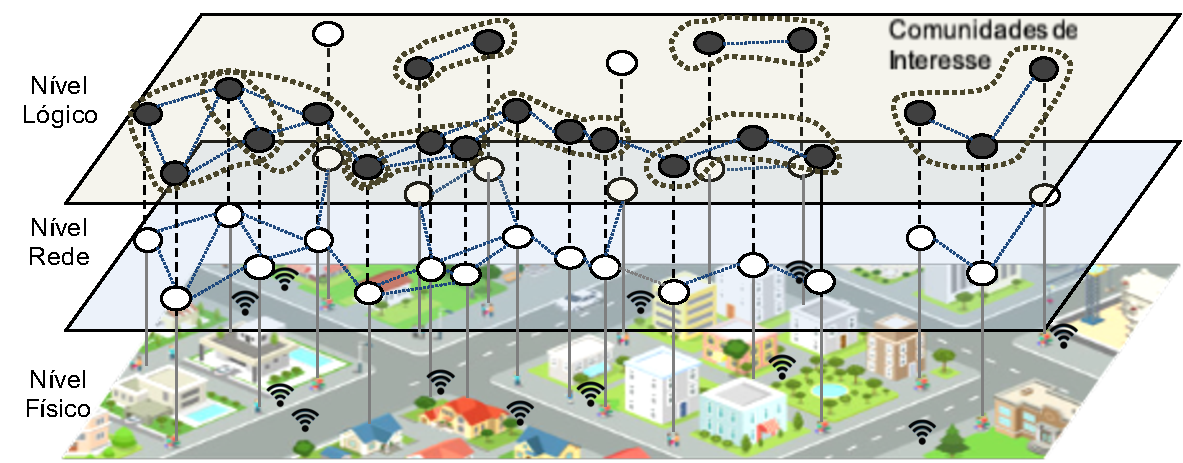
\includegraphics[width=1\textwidth]{figures/ModeloRede.pdf}
\caption{Modelo de Rede}
\label{fig:modeloRede}
\end{figure}
\end{minipage}
\begin{minipage}[b]{.52\linewidth}
\begin{figure}[H]
\centering
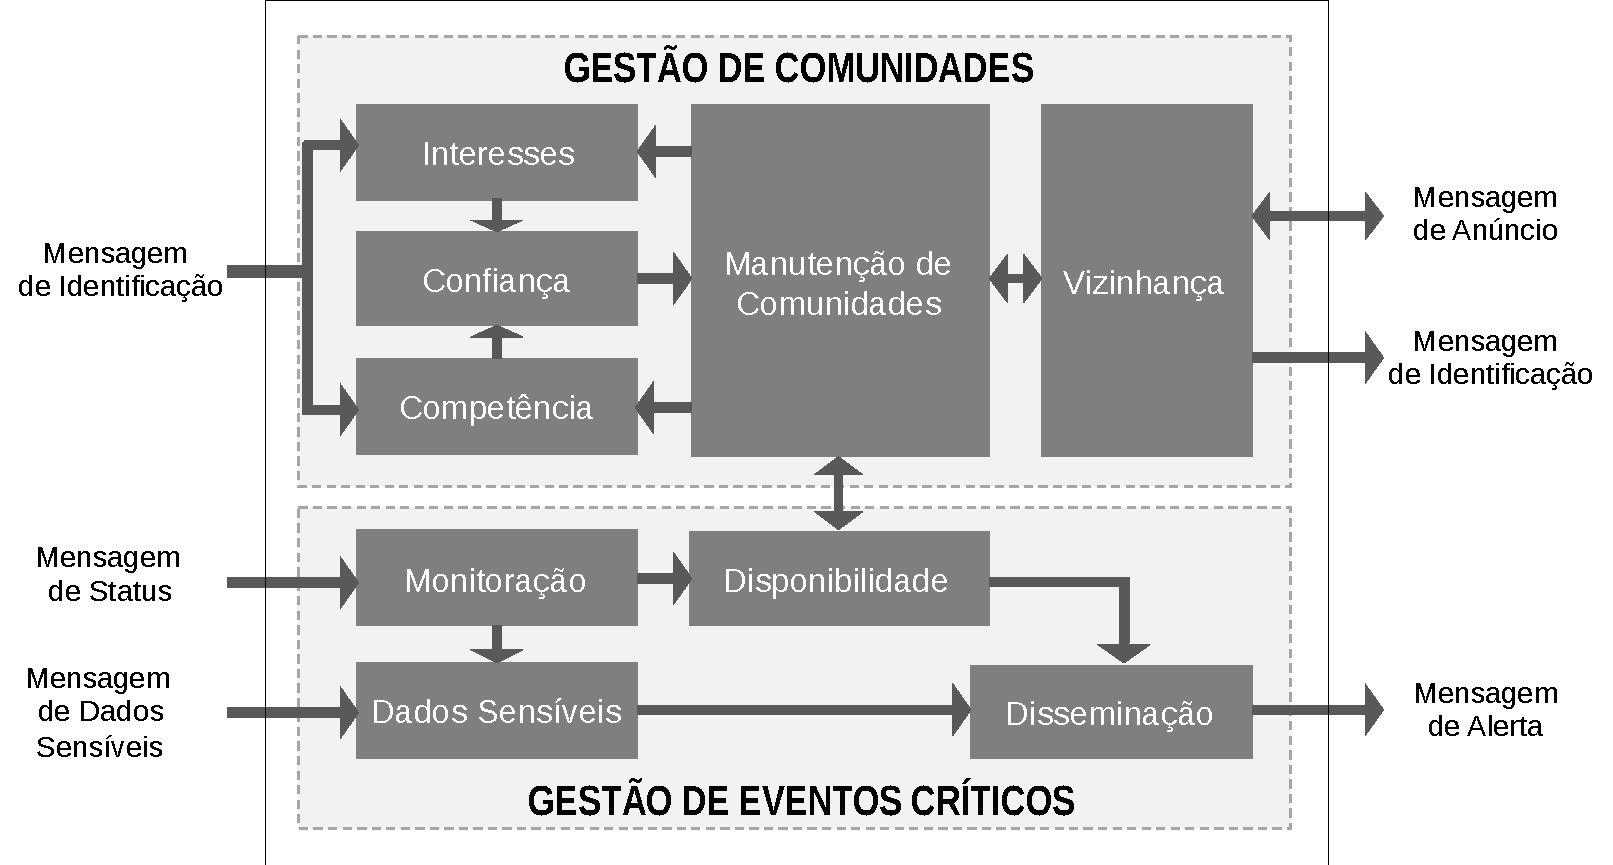
\includegraphics[width=1\textwidth]{figures/Arquitetura_8_p.pdf}
\caption{Arquitetura do \mbox{STEALTH}}
\label{fig:ArquiteturaStealth}
\end{figure}
\end{minipage}

O funcionamento do \mbox{STEALTH} inicia com
\agn{a operação dos}
%os 
nós da rede
%operando de 
forma isolada e, na medida em que se movimentam, encontram outros nós e estabelecem comunidades de interesse. Periodicamente, cada nó inicializa sua lista de vizinhos, anuncia sua presença por mensagens de anúncios em \textit{broadcast} à procura de nós vizinhos e aguarda um intervalo de tempo até um novo anúncio.  Quando um nó vizinho percebe que um nó anuncia a sua presença, encaminha a este nó anunciador uma mensagem de identificação, composta pela seu \textit{Id}, competência e interesses. O nó anunciador, ao receber essa mensagem do nó vizinho, verifica a existência de interesse em comum em saúde entre eles. Quando há esse interesse, ele mede a confiança do nó vizinho e o insere na sua lista de vizinhos, dentro da sua comunidade de saúde. A partir dessa confiança~(Eq.~\ref{eq:communityTrust}) e da sua competência~(Eq.~\ref{eq:SkillTrust}), obtém-se a confiança total do nó~(Eq.~\ref{eq:totalTrust}). 
%Nas situações emergenciais de saúde, os nós pertencentes às CoI em saúde apoiam os nós que representam pessoas em situação emergencial.
Assim, ao ocorrer um evento crítico com um nó, este nó determina o nó vizinho que ele mais confia, e o dado sensível apropriado a ser disseminado. Em seguida, ele envia uma mensagem de alerta ao nó selecionado com seu dado sensível, e anuncia aos nós a interrupção de sua operação. Ao receber uma mensagem de alerta, o nó confirma seu recebimento.
%Quando um nó percebe que outro nó anuncia a interrupção de sua operação, ele exclui esse nó da sua lista de vizinhos. Isso impede que um nó em situação emergencial seja selecionado para receber dados sensíveis de outros nós. 


\vspace{-0.5cm}

\noindent
\begin{minipage}{.3\linewidth}
\centering
\begin{equation}
T_{xy}^{I} = \frac {|I_x \cap I_y|}{|I_x|}
\label{eq:communityTrust}
\end{equation}
\end{minipage}
\begin{minipage}{.3\linewidth}
\centering
\begin{equation}
T_{xy}^{Skill} = Sim_y
\label{eq:SkillTrust}
\end{equation}
\end{minipage}
\hspace{0.5cm}
\begin{minipage}{.3\linewidth}
\centering
\begin{equation}
T_{xy} = \frac{T_{xy}^{I} + T_{xy}^{Skill}}{2}
\label{eq:totalTrust}
\end{equation}
\end{minipage}


%Nós ilustramos a operação do \mbox{STEALTH} em um ambiente urbano de modo a apoiar uma pessoa em situação emergencial, a fim de que ela possa receber um primeiro atendimento. 
Considere uma área urbana onde seis pessoas deslocam-se a pé pelas ruas.
%: uma enfermeira, um paciente, um executivo, um policial, um bombeiro e um médico.
%Cada uma delas possui uma profissão ou habilidade para executar determinadas tarefas no seu dia-a-dia. 
%O paciente é uma pessoa que eventualmente precisa de atendimento emergencial.
%O médico detém o maior conhecimento em saúde e o policial, por exemplo, possui condições de prestar primeiros socorros. 
Todas essas pessoas possuem um interesse em comum em saúde e não mantêm relações entre si, mas podem estabelecer {\bf redes locais dinâmicas} em razão da sua proximidade e do interesse em saúde. %As pessoas portam dispositivos móveis, \textit{smartphones}, para se conectarem em redes. 
O \mbox{STEALTH} roda nesses \textit{smartphones}. Além disso, o paciente porta um dispositivo junto ao seu corpo para verificar sua pressão arterial, por exemplo, e reportar a um aplicativo instalado em seu \textit{smartphone}. Esse aplicativo
%comunica-se com o 
\agn{informa ao}
\mbox{STEALTH}
%para informar 
os valores de pressão arterial medidos e sua normalidade para esse paciente.


\begin{table}[!htb]
	\begin{minipage}[t]{0.5\linewidth}
		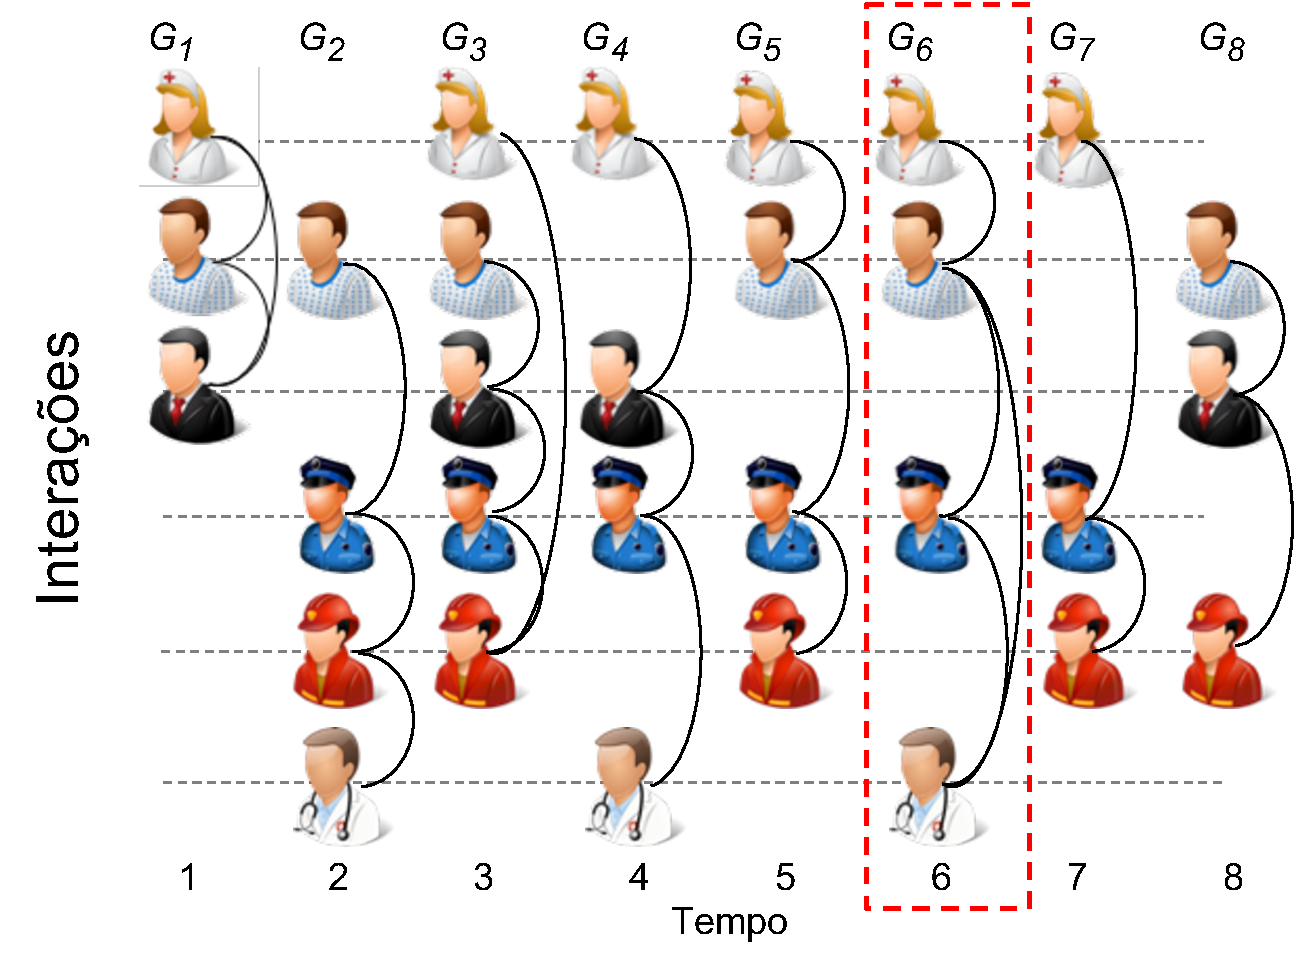
\includegraphics[width=0.95\textwidth]{figures/interacoes_t6.pdf}
		\captionof{figure}{Interações no tempo}
		\label{fig:interacoesnotempo}
	\end{minipage}
	\begin{minipage}[b]{0.5\linewidth}
		\centering
		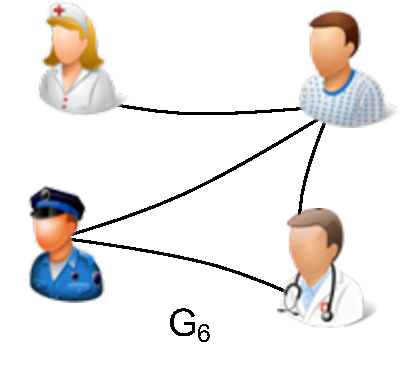
\includegraphics[width=.3\textwidth]{figures/Grafo6.pdf}
		\vspace{-0.2cm}
		\captionof{figure}{Grafo da rede em $t_6$}
	    \label{fig:grafo6}
	    \relsize{-2.0}
	    \captionof{table}{Medição da confiança}
        \label{tab:exemploConfianca2}
        {
            \begin{tabular}{|l|ccc|}
            \hline%B{2}
            \multirow{2}{*}{\textbf{Confiança}}&\multicolumn{3}{c|}{\textbf{Competência}}  \\ \cline{2-4}
            &Médico&Enfermeira&Policial  \\ \hline
            \textbf{$T^{Skill}$}&1&0,33&0,28 \\
            \textbf{$T^{CoI}$}&1&1&1  \\
            \textbf{$T$}&1&0,66&0,64 \\
            \hline%B{2}
            \end{tabular}
        }
	\end{minipage}\hfill
\end{table}

As interações entre pessoas ao longo do tempo $t = \{1,2,...,8\}$
%, resultantes da sua mobilidade, 
estabelecem redes locais, ilustradas na Figura \ref{fig:interacoesnotempo}, quando seus dispositivos estabelecem redes \textit{ad hoc} para trocarem dados entre si. Assume-se que o paciente entra em uma situação emergencial em $t_6$. Nesse instante, o seu dispositivo interage com os de outras pessoas próximas, como ilustra o grafo temporal $G_6$ (Figura \ref{fig:grafo6}), e cada um deles forma sua própria comunidade de saúde. O dispositivo do paciente mede a confiança dos demais e os insere entre os seus vizinhos com os valores de confiança exibidos na  Tabela~\ref{tab:exemploConfianca2}. Ao ocorrer o evento crítico em $t_6$, o \mbox{STEALTH} rodando no \textit{smartphone} do paciente recomenda o médico como o maior valor de confiança na sua comunidade de saúde e, assim, dissemina seus dados sensíveis para que ele possa adotar alguma ação.

\section{Avaliação} \label{sec:aval}

O sistema \mbox{STEALTH} foi implementado e simulado no simulador NS-3, versão 3.28.\footnote{Código disponível em https://github.com/agnaldosb/stealth} Todos os resultados correspondem à média de 35 simulações, com intervalo de confiança de 95\%. A análise da disponibilidade dos dados provida pelo \mbox{STEALTH} levou em conta a evolução das comunidades de interesse em saúde ao longo do tempo e a métrica \textit{Número médio de comunidades de interesse em saúde}~($N_{C}$). A
\agn{mensuração da}
análise da confiabilidade
%é mensurada 
\agn{ocorre}
através das métricas \textit{Taxa de sucesso no acesso aos dados}~($TS$), \textit{Taxa de dados não acessados}~($TN_a$), \textit{Tempo médico de acesso aos dados}~($MTA$) e \textit{Taxa de sucesso no acesso aos dados por competência}~($TS_{Skill}$). Os parâmetros empregados nas simulações, bem como todos os resultados obtidos estão na dissertação.

\begin{table}[H]
\setlength{\extrarowheight}{2.0pt}
\relsize{-2.0}
\centering
\caption{Distribuição dos aspectos sociais atribuídos aos nós}
\vspace{-0.2cm}
\label{tab:aspectosAtribuidos}
\begin{tabular}{|l|cccc|ccccc|}
\hline%B{2}
\multirow{2}{*}{\textbf{Aspectos Sociais}} & \multicolumn{4}{c|}{\textbf{Competências}} & \multicolumn{5}{c|}{\textbf{Interesses}} \\ \cline{2-10}
&Médico&Enfermeiro&Cuidador&Outras&Saúde&Turismo&Música&Filmes&Livros \\ \hline
\textbf{\# de Nós} &10&15&20&55&20&30&45&60&15 \\ 
\hline%B{2}
\end{tabular}
\end{table}

Os nós da rede foram configurados randomicamente com aspectos sociais a cada repetição de simulação, conforme Tabela~\ref{tab:aspectosAtribuidos},
%possuindo 
\agn{para possuírem}
uma única competência e um conjunto de interesses, com um mínimo de um e máximo cinco interesses. A avaliação do~sistema foi realizada por meio dos nós 37, 52 e 70.
%Cada um desses nós recebeu a mesma configuração em todas as repetições de simulações e entrou em situação emergencial aos 890s. 
Assumiu-se que todos os nós possuem um comportamento honesto e há mecanismos de segurança para validar suas identidades e proteção na transmissão dos dados. Além disso, 
%Assume-se, que 
o alerta de um evento crítico~acontece por 
%meio de 
um dispositivo portado pelas pessoas junto ao 
corpo, e que informa ao~\mbox{STEALTH}.



\section{Disponibilidade e Confiabilidade} \label{sec:results}

\begin{wrapfigure}{r}{0.35\textwidth}
\centering
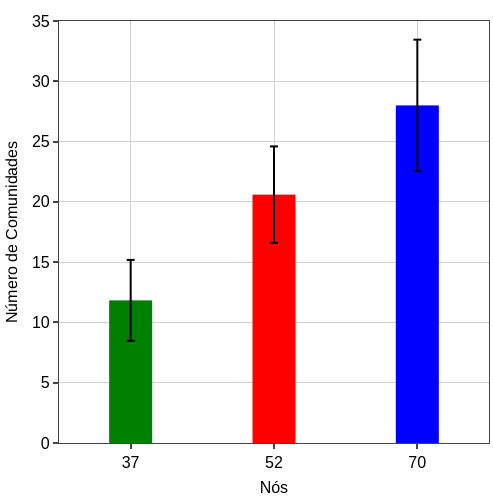
\includegraphics[width=.35\textwidth]{figures/coi_mean_performance_3_SBSEG19_v2.png}
\vspace{-0.5cm}
\caption[Número médio de comunidades]
{\tabular[t]{@{}l@{}}Número médio de \\ comunidades\endtabular}
\label{fig:coiEstabelecidas}
\end{wrapfigure}    

A disponibilidade do \mbox{STEALTH} representa sua prontidão para disseminar com sucesso e de modo controlado os dados sensíveis das pessoas em situação emergencial. O número médio de comunidades de interesse em saúde ($N_{C}$) demonstra esse comportamento (Figura~\ref{fig:coiEstabelecidas}).
%O 
\agn{As CoI formadas pelo}
nó 37,
%estabeleceu, 
em média, 12 CoI em cada repetição de simulação,
%caracterizando 
\agn{caracterizam}
a dinamicidade das redes locais estabelecidas e de sua topologia. A mobilidade dos nós, associada aos seus aspectos sociais (interesses), impactou a formação das comunidades.
%O nó 70 estabeleceu uma quantidade maior de comunidades, $N_C$ = 28, elevando a disponibilidade para disseminação de seus dados em situações emergenciais.
%
%
%A evolução das comunidades de saúde dos nós 37, 52 e 70, estabelecidas pelo \mbox{STEALTH} em uma repetição específica de simulação, é ilustrada na Figura~\ref{fig:neighs_x_cois}. 
O \mbox{STEALTH} acompanhou a dinamicidade das redes locais criadas diante da mobilidade dos nós,
%ajustando 
\agn{e ajustou}
suas CoI \agn{(Figura~\ref{fig:neighs_x_cois}).}
%O nó 37 formou comunidades em 63,93\% do tempo em que esteve ativo. Nesse período, o sistema esteve apto para disseminar seus dados sensíveis.
%, pois  identificou  vizinhos que poderiam auxiliá-lo. 
%Contudo, ao entrar em emergência aos 890s, o nó 37 não possuía vizinhos ao redor, impedindo a formação de uma comunidade e  a disseminação de seus dados sensíveis. 
%O 
\agn{Em uma repetição da simulação, o}
nó 52
manteve um comportamento distinto e estabeleceu comunidades em 97,22\% do tempo, até que entrou em situação emergencial. Neste instante,
%como se observa na Figura~\ref{fig:neighs_x_cois}, 
ele possuía sete vizinhos, mas apenas dois deles pertenciam a sua comunidade de saúde (i.e., nós 13 e 41). Em razão do nó 13 possuir  uma competência mais elevada em saúde, \textit{cuidador}, o nó 52 disseminou seus dados para ele.
%Já  
%\agn{Por outro lado,}
%o nó 70  formou comunidades de saúde por mais tempo, 98,8\%.
%Esse comportamento é confirmado pela Figura~\ref{fig:coiEstabelecidas}, onde o nó 37 estabeleceu o menor $N_C$, 12, e o nó 70 teve o maior valor entre todos os nós, 28. Ao entrar em emergência, o nó 70 tinha 4 vizinhos, mas apenas um deles com interesse em saúde - nó 96, para o qual seus dados sensíveis foram disseminados. 

\begin{figure}[!htb]
\centering
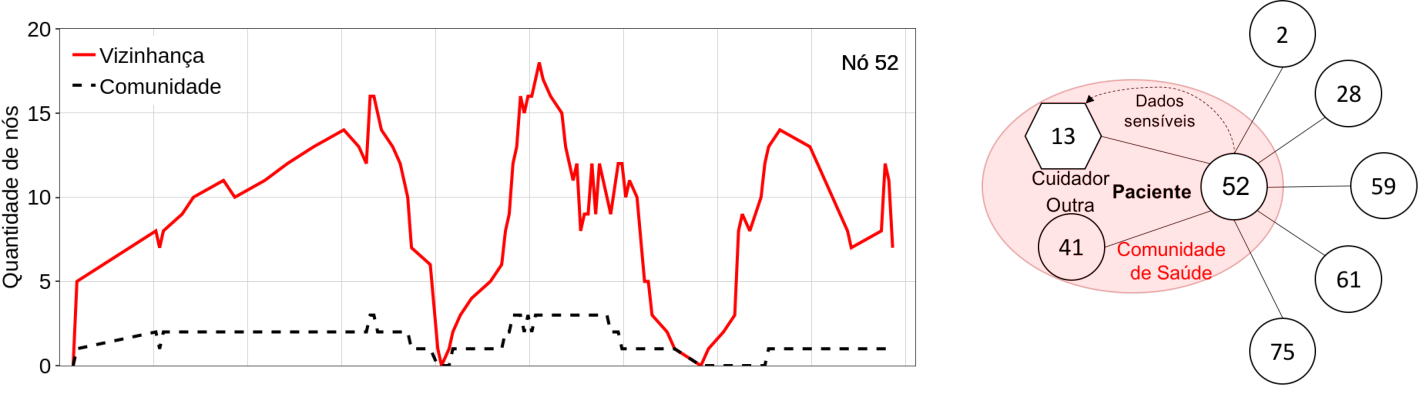
\includegraphics[width=0.9\textwidth]{figures/neighs_cois_v2_890s_stack_1node.pdf}
%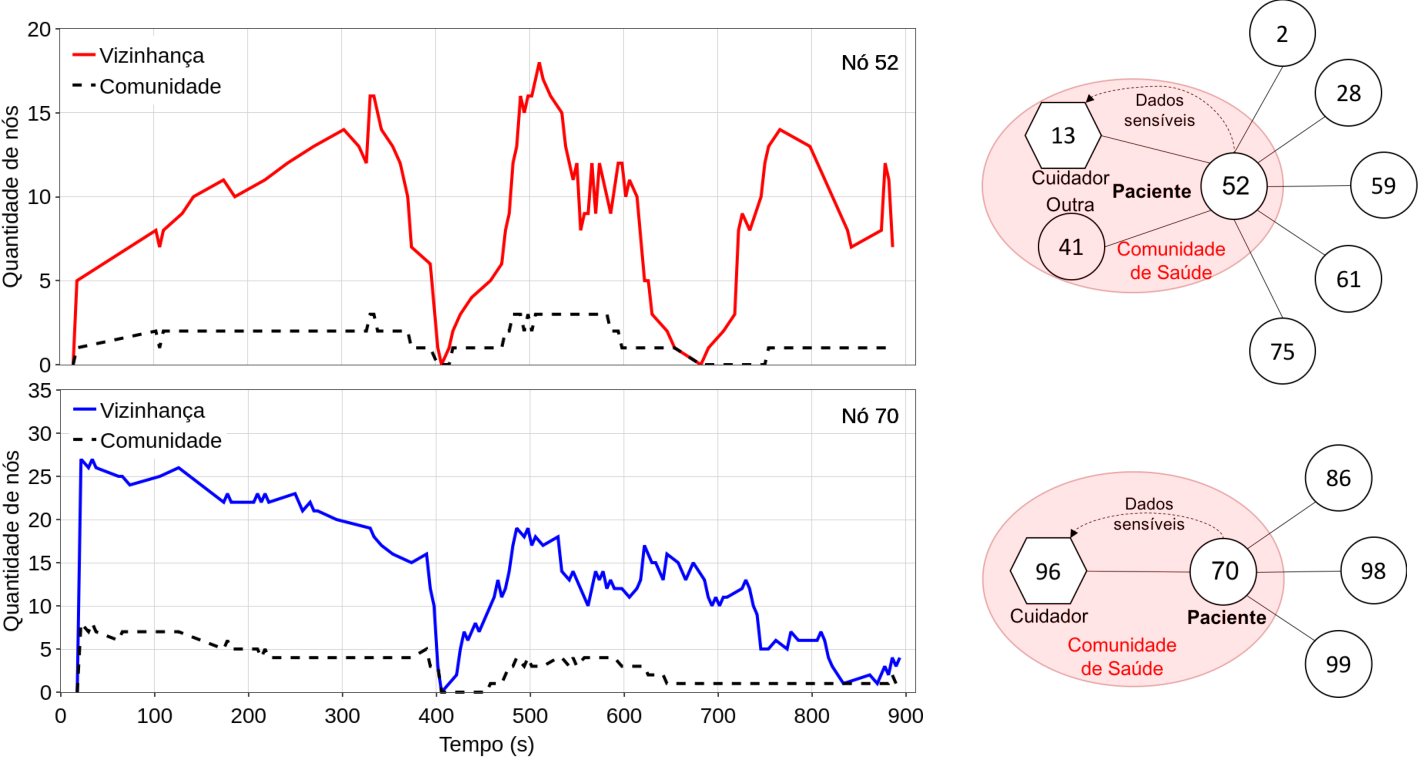
\includegraphics[width=0.9\textwidth]{figures/neighs_cois_v2_890s_stack_2nodes.pdf}
\vspace{-0.2cm}
\caption{Dinamicidade e tamanho da comunidade de saúde ao longo do tempo}
\label{fig:neighs_x_cois}
\end{figure}


A análise da confiabilidade leva em conta a capacidade do sistema em disseminar com sucesso e de modo controlado os dados sensíveis das pessoas em situação emergencial. O nó 52 foi bem-sucedido ($TS$) na disseminação de seus dados sensíveis em 80\% das situações emergenciais ao longo das repetições de simulações.
%O agrupamento dos nós em comunidades de interesse impacta a $TS$, pois garante a disseminação dos dados sensíveis de um nó em situação emergencial apenas a um outro nó dentre aqueles pertencentes a sua CoI em saúde. 
\agn{Os dados não acessados ($TNa$) permitem constatar a}
%A 
importância das comunidades no controle da disseminação desses dados.
%é constatada pelos dados não acessados ($TNa$). 
Os dados sensíveis do nó 37 não foram acessados em 68,57\% das situações emergenciais
%. Isso se deve 
\agn{devido}
à falta de uma comunidade de saúde
%durante as situações emergenciais 
ou a sua mobilidade, que interrompeu a conexão com os outros nós da sua rede local. O nó 70 não foi tão bem-sucedido
%quanto o nó 52, apesar de ter estabelecido um maior número de comunidades, como visto na Figura~\ref{fig:coiEstabelecidas}. Isto se deve à
\agn{diante da ausência}
%falta 
de vizinhos no instante em que
%o nó 70 
entrou em situação emergencial.
%nas repetições de simulações.
%A ausência de vizinhos para formar uma comunidade de saúde tornou a disseminação de seus dados sensíveis inviável. 
O
%tempo médio de acesso aos dados sensíveis
%(\textbf{
$MTA$
%}) 
representa o custo em relação ao tempo de acesso aos dados sensíveis de um nó.
%para que os dados sensíveis disseminados por um nó em situação emergencial sejam acessados. 
A dinamicidade das redes locais estabelecidas impacta o \textbf{$MTA$}, visto que a mobilidade dos nós impõe mudanças à topologia dessas redes. Os resultados na Tabela~\ref{tab:AcessoCompetencia} demonstram que o \mbox{STEALTH}
%dissemina dados sensíveis atendendo 
\agn{atende}
à latência máxima de 125ms estabelecida pela IEEE para entrega de alertas médicos~\cite{ieee2012}. O acesso aos dados sensíveis do nó 52 deu-se mais rapidamente que para os dos demais nós ($MTA$~<~1ms), já os do nó 37 foram acessados, em média, após 95ms de sua disseminação. 
%As CoI contribuem nas tomadas de decisões acerca do nó adequado que terá acesso aos dados disseminados, além de reduzirem o tempo de acesso a esses dados.

\begin{table}[!htb]
	\begin{minipage}[t]{0.5\linewidth}
	    \centering
        \caption{Disseminação dos dados}
        \vspace{-0.2cm}
        \label{tab:AcessoCompetencia}
        { \footnotesize
        \begin{tabular}{l|c|ccc}
        \hline%B{2}
        \multicolumn{2}{l|}{\textbf{Métrica}} & $TS$ &$TN_a$& $MTA$\\ \hline% \bigstrut \\ \hline %\hline
        \multirow{3}{*}{\textbf{Nó}}&37 & 31,43\% &\textcolor{blue}{\textbf{68,57}\%}& \textcolor{blue}{\textbf{95 ms}}\\% \bigstrut \\ 
        &52 & \textcolor{blue}{\textbf{80,00}\%} &20,00\% & < 1ms\\% \bigstrut \\
        &70 & 60,00\% &40,00\% &2,3 ms \\% \bigstrut \\ 
        \hline%B{2}
        \end{tabular}
        }
	\end{minipage}	
	\begin{minipage}[t]{0.5\linewidth}
	    \centering
	    \relsize{-2.0}
        \caption{Controle de disseminação}
        \vspace{-0.2cm}
        \label{tab:taxaMedia}
        { \footnotesize
        \begin{tabular}{l|c|c}
        \hline%B{2}
        \multicolumn{2}{l|}{\textbf{Métrica}} & $TS_{Skill}$ \\ \hline% \bigstrut \\ \hline
        \multirow{4}{*}{\textbf{Competência}}&Médico & 30,03\% \\% \bigstrut \\
        &Enfermeiro & 39,40\% \\% \bigstrut \\
        &Cuidador & 9,09\% \\% \bigstrut \\ 
        \hline%B{2}
        \end{tabular}
        }
	\end{minipage}\hfill
\end{table}

\vspace{0.3cm}

%Os dados sensíveis dos nós em situação emergencial foram disseminados pelo \mbox{STEALTH} apenas aos nós pertencentes as suas comunidades de saúde e diante das competências vistas na Tabela~\ref{tab:aspectosAtribuidos}. 
Os interesses e competências, associados às comunidades de interesse, além de possibilitarem avaliar a confiança dos nós, também permitem controlar a disseminação dos seus dados sensíveis. Isso ocorre em uma condição \textit{Zero-Knowledge},
%visto que as comunidades de saúde são recriadas periodicamente, 
visto a recriação periódica das comunidades de saúde.
e desconsidera interações anteriores entre os nós da rede. O sucesso no acesso aos dados por competência ($TS_{Skill}$) comprova a importância das competências nas comunidades estabelecidas. Através da Tabela~\ref{tab:taxaMedia}, observa-se que os \textit{médicos} acessaram os dados sensíveis em 30,03\% das situações emergenciais. Nesses momentos, o \mbox{STEALTH} detectou a presença de pelo menos um \textit{médico} na comunidade de saúde dos nós avaliados.

\vspace{-0.2cm}

\section{Conclusão}
\label{sec:conc}

Esta dissertação apresentou \mbox{STEALTH}, um sistema para disseminar dados sensíveis de saúde de forma controlada em redes locais dinâmicas sem fio. Ele estabelece agrupamentos virtuais por meio de comunidades de interesses e aplica confiança social a fim de permitir aos dispositivos decidirem de maneira robusta num dado momento sobre a disseminação de dados diante de uma situação emergencial. Uma avaliação do \mbox{STEALTH} num ambiente realístico mostrou a sua eficácia ao antecipar a identificação de pessoas próximas para auxiliar em eventos críticos de saúde, e sua confiabilidade na disseminação controlada dos dados sensíveis das pessoas em situação emergencial. As contribuições deste trabalho resultaram na publicação~\cite{batista2019sbseg}.

\small
\bibliographystyle{sbc}
\bibliography{CTD-CSBC2020}

\end{document}

